\section{Zielsetzung}
In diesem Versuch soll durch eine Röntgenreflektivitätsmessung (XSR: X-Ray Specluar Reflection) die Dichte, Schichtdicke und die
Rauigkeit einer dünnen Polystyrolschicht auf einem Silizium-Wafer bestimt werden.
Für diese Messung wird ein Oberflächendiffraktometer (Reflektometer) der Firma Bruker-AXS
verwendet.

\section{Theorie}
\subsection{Grundlagen der Röntgenreflektivität}
Bei der Röntgenreflektivität wird das zu untersuchende Medium mit Röntgenstrahlung einer Wellenlänge von
$\lambda=\SI{0,1}{\angstrom}$ bis $\SI{10}{\angstrom}$ bestrahlt. Der Einfallswinkel wird dabei so
gewählt, dass es an der Oberfläche zu einer Totalreflexion kommt.
Diese tritt für Röntgenstrahlung bei sehr kleinen Winkeln bezogen auf die Oberfläche auf, da der Realteil
des Brechungsindex für Röntgenstrahlung <1 ist. Dies ergibt sich aus der allgemeinen Darstellung des Brechungsindex
über
\begin{equation}
  n=1-\delta+i\beta.
\end{equation}
mit den Größenordnungen $\delta\approx \SI{10e-6}{}$ und $\beta\approx\SI{10e-7}{}$(für $E=\SI{8}{\keV}$).
Der Imaginärteil mit dem Koeffizienten $\beta$ bestimmt dabei die Absorption.

\begin{figure}
  \centering
  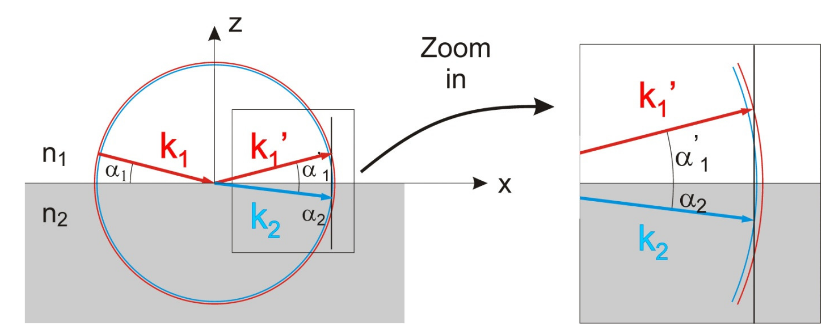
\includegraphics[width=8cm]{Brechung.png}
  \caption{Schematische Darstellung für die Brechung von Röntgenstrahlen an einer Grenzfläche \cite{XSR}.}
  \label{}
\end{figure}

Nach dem Snellius'schen Brechungsgesetz
\begin{equation}
  \frac{cos\alpha_1}{\cos\alpha_2}=\frac{n_2}{n_1}
  %n_1\cos(\alpha_2)=n_2\cos(\alpha_1)
\end{equation}
ergibt sich für $Re(n_2)<1$, dass der transmittierte Strahl vom Lot weggebrochen wird, wodurch es zu
einem kritischen Winkel $\alpha_c$ kommt, unterhalb dessen keine transmittierte Welle mehr auftritt und
Totalreflexion vorliegt.

Unter Vernachlässigung der Absorpion, also für $\beta=0$, ergibt sich
\begin{equation}
  a_c\approx \lambda\sqrt{\frac{r_e \rho}{\pi}}
  \label{eqn:alphac}
\end{equation}
mit der (Elektronen)dichte des Materials $\rho$ und dem Elektronenradius $r_e$.

\subsection{Fresnelformeln}
Kommt es zur Brechung elektromagnetischer Wellen an einer Oberfläche können der Reflexions- und
Transmissionskoeffizient über die Fresnelformeln bestimmt werden. Im Allgemeinen unterscheiden
sich diese für s- und p-polarisierte Strahlung. Für den Fall kleiner Einfallswinkel, welcher in diesem Versuch
vorliegt, ist dieser Unterschied vernachlässigbar klein.
Somit gilt für den Reflexions- und Transmittionskoeffiziet:
\begin{align}
 r=\frac{n_1cos \alpha_1 -n_2 \cos\alpha_2}{n_1\cos\alpha_1 + n_2 \cos\alpha_2}\;\;\; \text{und}\;\;\; t=\frac{2n_1 \cos\alpha_1}{n_1\cos\alpha_1 + n_2 \cos\alpha_2}
\end{align}

Aus dem Reflexionskoeffizient lässt sich nach $R=|r^2|$ die Fresnelreflektivität berechnen, welche sich
für $\alpha_1>3\alpha_c$ näherungsweise zu
\begin{equation}
  R_F=\Big(\frac{\alpha_c}{2\alpha_i} \Big)^4
  \label{eqn:reflektivität}
\end{equation}
ergibt. Ein schematischer Kurvenverlauf der Relexivität in Abhängigkeit des Einfallswinkels ist in
Abbildung \ref{fig:reflex} dargestellt. Wie nach Formel \ref{eqn:reflektivität} zu erwarten, ist mit steigendem
Einfallswinkel ein starker Abfall der Reflektivität zu beobachten, welcher proportional zu $(\alpha_1)^{-4}$ ist.

\begin{figure}
  \centering
  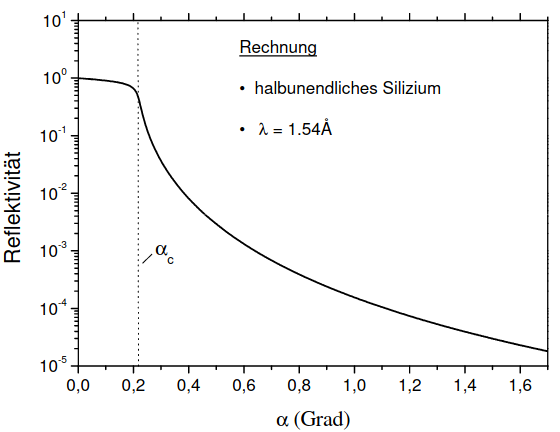
\includegraphics[width=9cm]{Reflektivität.png}
  \caption{Reflektivität von Silizium in Abhängigkeit des Winkels \cite{XSR}.}
  \label{fig:reflex}
\end{figure}


\subsection{Röntgenreflektivität an mehreren Schichten}
Im Folgenden wird ein System aus zwei Schichten, einem Substrat und einem Adsorbat betrachtet, sodass es sowohl an der
Vakuum/Adsorbat-, als auch an der Adsorbat/Substrat-Grenzfläche zur Brechung kommt. Dieses System ist schematisch in
Abbildung \ref{fig:mehr} dargestellt.

\begin{figure}
  \centering
  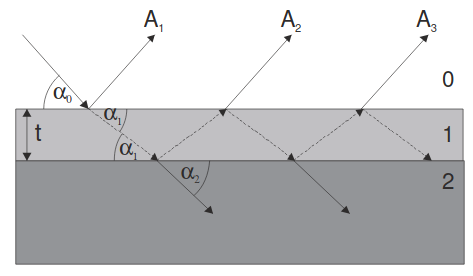
\includegraphics[width=7cm]{Medium.png}
  \caption{Schematische Darstellung einer Zweischichtprobe, bestehend aus Substrat und Adsorbat, welche mit
  Röntgenstrahlung bestrahlt wird \cite{XSR}.}
  \label{fig:mehr}
\end{figure}

Da die reflektierten Wellen sowohl an der Vakuum/Adsorbat-, als auch an der Adsorbat/Substrat-Grenzfläche konstruktiv,
als auch destruktiv interferieren können, kommt es zu Oszillationen in der Fresnelreflektivität.
Für einen $\SI{800}{\angstrom}$ dicken Polystyrolfilm auf einer Siliziumoberfläche sind diese Oszillationen, welche
auch als Kiessig-Oszillationen bekannt sind, in Diagramm \ref{fig:Kiessig} dargestellt. Zusätzlich ist ein Einschub mit den
für Einfallswinkel $<\SI{0,4}{\degree}$ dargestellt, welcher die kritischen Winkel $\alpha_c$ für Silizium und
Polystyrol zeigt.

\begin{figure}
  \centering
  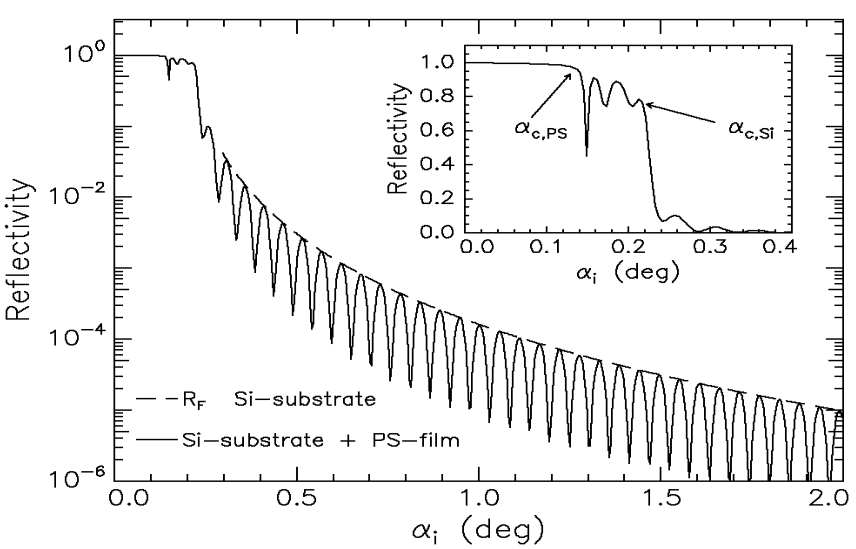
\includegraphics[width=10cm]{Kiessig.png}
  \caption{Röntgenreflektivität einer $\SI{800}{\angstrom}$ dicken Polystyrolschicht auf einem Siliziumsubstrat.
  Deutlich zu erkennen sind sowol der starke Intensitätsabfall für große Einfallswinkel, als auch die Kiessig-Oszillation \cite{skript}.}
  \label{fig:Kiessig}
\end{figure}

Mithilfe dieser Oszillationen lassen sich Rückschlüsse auf den Schichtabstand ziehen, denn für destruktive Interferenz
muss der Gangunterschied ein ungerades Vielfaches der halben Wellenlänge $\frac{\lambda}{2}$ sein.
Daraus lässt sich der Zusammenhang
\begin{equation}
  d=\frac{2\pi}{\delta q_z}=\frac{\lambda}{2\delta\alpha_1}
  \label{eqn:dicke}
\end{equation}
mit dem Wellenvektorübertrag $\vec{q}=\vec{k_2}-\vec{k_1}$ und der z-Komponente $q_z=2k\sin(\alpha_1)$ bestimmen. Dieser ist in Abbildung \ref{fig:Streuvek} anschaulich
dargestellt.

\begin{figure}
  \centering
  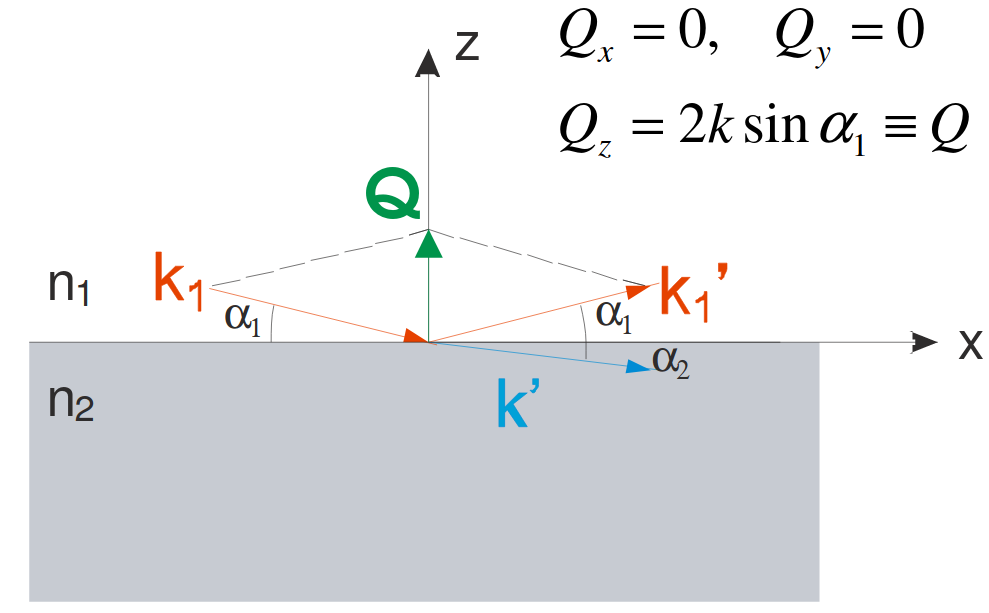
\includegraphics[width=6cm]{Streuvek.png}
  \caption{Darstellung des Streuvektors \cite{XSR}.}
  \label{fig:Streuvek}
\end{figure}


Wird nun ein System aus mehr als zwei Schichten betrachtet, wie es in Abbildung \ref{fig:mehrschicht} dargestellt ist, überlagern
sich die die verschiedenen Oszillationen und es ergibt sich eine kompliziertere Reflektivität. Diese lässt sich über den rekursiven
Parratt-Algorithmus berechnen, welcher darauf basiert, dass die unterste Schicht als unendlich dick angenommen wird und es somit zu keiner
Reflextion, sondern nur zu Transmission kommt.
Auf dieser Grundlage kann das Amplitudenverhältnis der reflektierten zur transmittierten Welle an der j-ten Grenzfläche geschrieben werden als
\begin{equation}
  X_j=\frac{R_j}{T_j}=\exp(-2ik_{z,j}z_j)\cdot\frac{r_{j,j+1}+X_{j+1}\exp(2ik_{z,j+1}z_j)}{1+r_{j,j+1}X_{j+1}\exp(2ik_{z,j+1}z_j)}
  \label{eqn:parratt}
\end{equation}
mit $r_{j,j+1}$ als Fresnelreflektivität der j-ten Grenzfläche.

\begin{figure}[H]
  \centering
  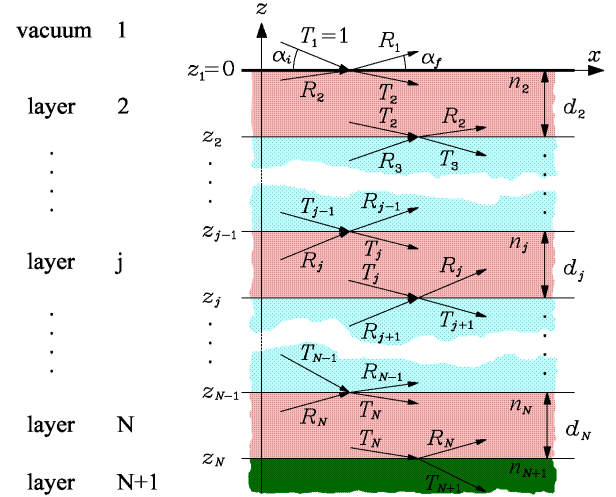
\includegraphics[width=8cm]{mehrschicht.png}
  \caption{Darstellung eines Mehrschichtsystems mit den jeweiligen Reflexions- und Transmissionskomponenten \cite{skript}.}
  \label{fig:mehrschicht}
\end{figure}

\subsection{Rauigkeit}
Da Oberflächen nie perfekt glatt sind, muss die Oberflächenrauigkeit bei der Berechnung der Reflektivität berücksichtigt werden. Dies
geschieht, indem die modifizierten Fresnelkoeffizienten
\begin{align}
  \tilde{r}_{j,j+1}&=r_{j,j+1}\exp(-2k_{z,j}k_{z,j+1}\sigma^2_j)\;\;\;\text{und}\\
  \tilde{t}_{j,j+1}&=t_{j,j+1}\exp((k_{z,j-k_{z,j+1}})^2\cdot\sfrac{\sigma^2_j}{2})
\end{align}
eingeführt werden. Dabei bezeichnet $\sigma_j$ die Rauigkeit der j-ten Schicht.
Der Einfluss der Oberflächenrauigkeit auf die Reflektivität ist in Abbildung \ref{fig:rau} veranschaulicht.

\begin{figure}
  \centering
  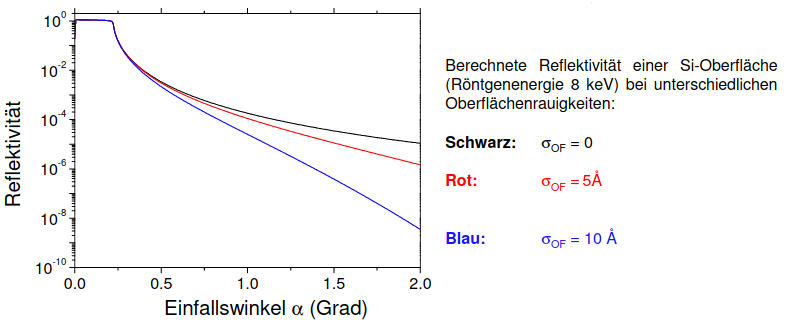
\includegraphics[width=13cm]{rau.png}
  \caption{Reflektivität einer Si-Oberfläche mit unterschiedlicher Oberflächenrauigkeit \cite{XSR}.}
  \label{fig:rau}
\end{figure}
